\documentclass[10pt,aspectratio=169]{beamer}
\usetheme{Madrid}
\usecolortheme{whale}
\setbeamertemplate{navigation symbols}{}
\setbeamertemplate{caption}{\insertcaption}
\usepackage{amsmath,amssymb}
\usepackage{graphicx}
\usepackage{booktabs}
\usepackage{tikz}
\usetikzlibrary{arrows.meta}

\title[Execution-Guided Self-Distillation]{Accelerating Test-Time Discovery in Complex Code Generation\\via Execution-Guided Self-Distillation}
\author[Mai Dang]{Mai Dang}
\institute[VNUHCM-US]{VNUHCM University of Science \\ \small Supervisor: \underline{\hspace{3cm}}}
\date{2026}

\begin{document}

% 1
\begin{frame}\titlepage\end{frame}

% 2
\begin{frame}{The problem}
\textbf{Test-time training (TTT):} fix one hard programming problem, let the model improve itself over a few inference-time steps, then reset.
\vfill
\begin{itemize}
  \item Reward is verifiable but \alert{sparse}: it only says \emph{whether} an attempt passed.
  \item On-policy self-distillation \alert{stalls} on hard problems --- the bare student rarely produces a correct attempt to learn from.
  \item This is the \textbf{flat-reward trap}: no correct rollout $\Rightarrow$ no usable gradient.
\end{itemize}
\vfill
\centering\emph{Goal: accelerate test-time \textbf{discovery} on complex code generation.}
\end{frame}

% 3
\begin{frame}{Background: SDPO and the gap}
\textbf{SDPO} (H\"ubotter et al.): extract a dense signal from the \emph{rich feedback} that verifiable environments already produce (failing tests, runtime errors).
\begin{itemize}
  \item The same model, conditioned on feedback, is a \textbf{self-teacher}; its per-token distribution is distilled into the student.
  \item Denser credit assignment than GRPO: a $K$-dim target per token, not one scalar per sequence.
\end{itemize}
\vfill
\textbf{The gap:} the parent method is \alert{student-first} --- it distills the student's \emph{own failed rollout}. On hard problems there is little that is correct to learn from.
\end{frame}

% 4
\begin{frame}{Our idea: teacher-first}
\centering
\scalebox{0.78}{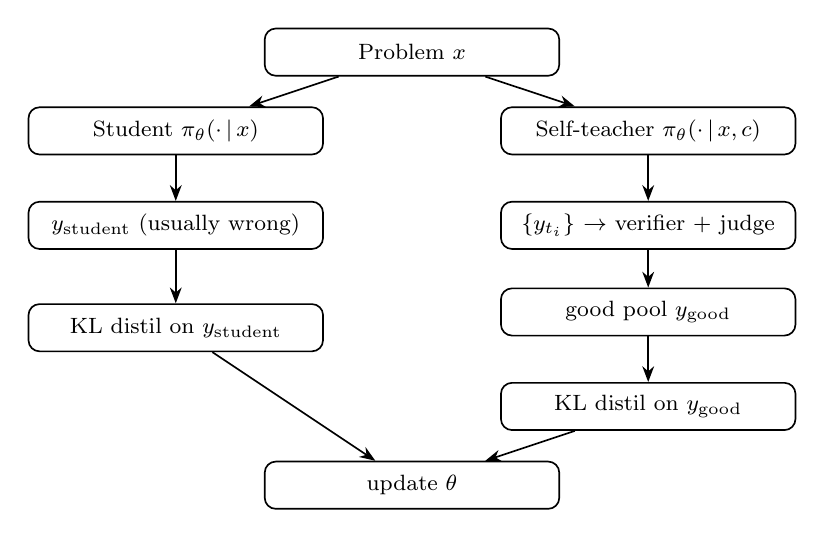
\begin{tikzpicture}[font=\footnotesize,>=Stealth,semithick,every node/.style={draw,rounded corners,align=center,minimum height=0.6cm,text width=3.6cm,inner sep=2pt}]
\node(x) at (3,5){Problem $x$};
\node(s) at (0,4){Student $\pi_\theta(\cdot\,|\,x)$};
\node(t) at (6,4){Self-teacher $\pi_\theta(\cdot\,|\,x,c)$};
\node(ys) at (0,2.8){$y_{\text{student}}$ (usually wrong)};
\node(yt) at (6,2.8){$\{y_{t_i}\}\to$ verifier + judge};
\node(g) at (6,1.7){good pool $y_{\text{good}}$};
\node(kls) at (0,1.5){KL distil on $y_{\text{student}}$};
\node(klt) at (6,0.5){KL distil on $y_{\text{good}}$};
\node(u) at (3,-0.5){update $\theta$};
\draw[->](x)--(s);\draw[->](x)--(t);\draw[->](s)--(ys);\draw[->](t)--(yt);\draw[->](yt)--(g);\draw[->](ys)--(kls);\draw[->](g)--(klt);\draw[->](kls)--(u);\draw[->](klt)--(u);
\end{tikzpicture}}
\vfill
{\small \textbf{Teacher-first:} distil a \emph{correct, filtered} trajectory the teacher generates --- between on-policy SDPO and off-policy SFT.}
\end{frame}

% 5
\begin{frame}{The teacher-first step}
\centering
\scalebox{0.82}{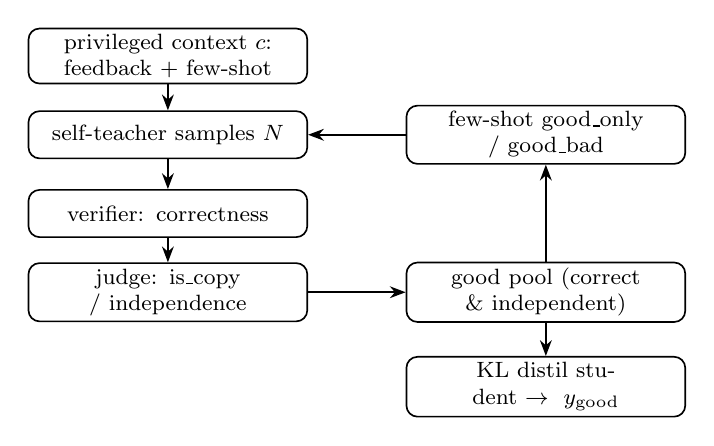
\begin{tikzpicture}[font=\footnotesize,>=Stealth,semithick,every node/.style={draw,rounded corners,align=center,minimum height=0.6cm,text width=3.4cm,inner sep=2pt}]
\node(c) at (0,4){privileged context $c$: feedback + few-shot};
\node(t) at (0,3){self-teacher samples $N$};
\node(v) at (0,2){verifier: correctness};
\node(j) at (0,1){judge: is\_copy / independence};
\node(gp) at (4.8,1){good pool (correct \& independent)};
\node(fs) at (4.8,3){few-shot good\_only / good\_bad};
\node(kl) at (4.8,-0.2){KL distil student $\to y_{\text{good}}$};
\draw[->](c)--(t);\draw[->](t)--(v);\draw[->](v)--(j);\draw[->](j)--(gp);\draw[->](gp)--(fs);\draw[->](fs)--(t);\draw[->](gp)--(kl);
\end{tikzpicture}}
\vfill
{\small Verifier $+$ judge filter for \emph{correct AND independent}; the filter never distils a copy (fallback removed).}
\end{frame}

% 6
\begin{frame}{Research questions}
\begin{itemize}
  \item[\textbf{RQ-method}] Does teacher-first beat student-first at discovering hard code solutions --- and does it survive at \emph{matched compute}?
  \item[\textbf{RQ1}] Does the \emph{reprompt-template} formulation of the feedback affect discovery?
  \item[\textbf{RQ2}] Does distillation from rich context \emph{suppress epistemic verbalization} on code?
  \item[\textbf{RQ3}] How does discovery trade off against \emph{compute} (compute-to-correct)?
\end{itemize}
\end{frame}

% 7
\begin{frame}{Setup}
\begin{itemize}
  \item Model: \textbf{Qwen3-4B} (LoRA), thinking ON; LiveCodeBench v6 (code), AIME 2026 (math pilot).
  \item Per problem: reset to base, \textbf{15 TTT steps}, evaluate student PRE vs POST.
  \item \textbf{8 frontier code problems $\times$ 6 seeds} (medium scale) $\Rightarrow$ Wilcoxon signed-rank test.
  \item Metrics: pass@16, discovery@k, total generations + GPU-time.
\end{itemize}
\end{frame}

% 8
\begin{frame}{RQ-method: teacher-first wins}
\begin{columns}
\column{0.6\textwidth}
\centering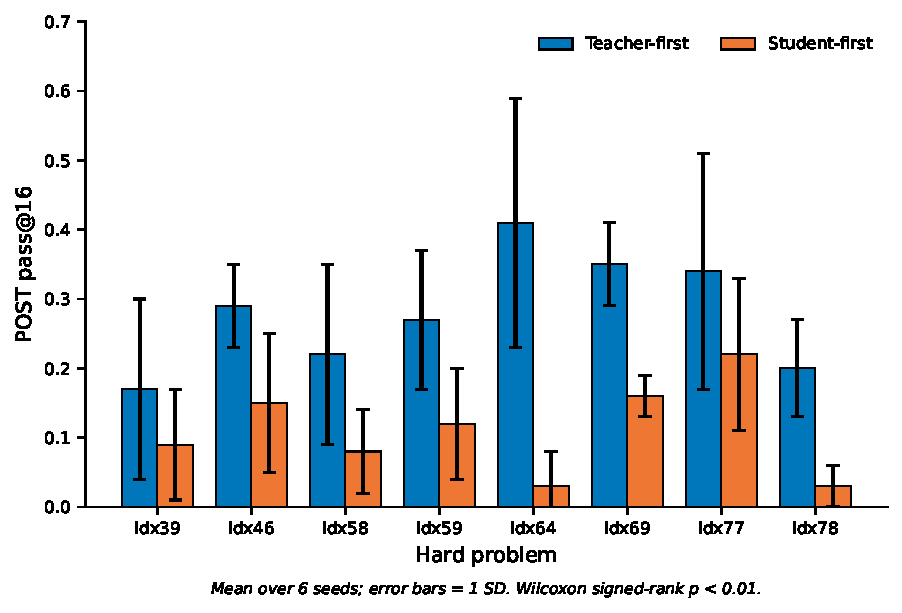
\includegraphics[width=\linewidth]{../figures/bc_fig1_main.pdf}
\column{0.4\textwidth}
\begin{itemize}
  \item TF $\geq$ SF on every problem, larger margins on the hardest.
  \item \alert{Wilcoxon $p<0.01$} (6 seeds) --- not a crude sign test.
  \item \textbf{RQ1:} on hard problems, template order \textbf{T5 $>$ T2 $>$ T1} (reasoning-inducing best).
\end{itemize}
\end{columns}
\end{frame}

% 9
\begin{frame}{The headline: escape-zero}
\begin{columns}
\column{0.6\textwidth}
\centering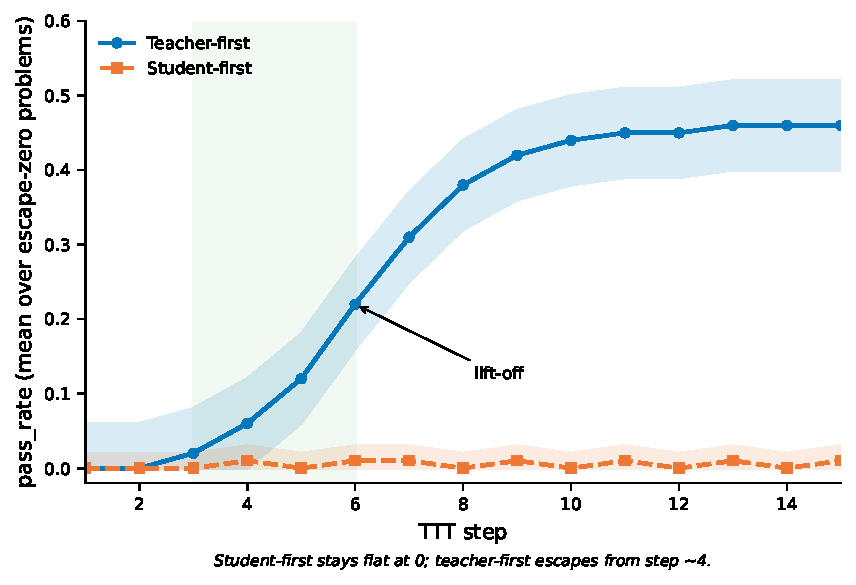
\includegraphics[width=\linewidth]{../figures/bc_fig2_discovery.pdf}
\column{0.4\textwidth}
\begin{itemize}
  \item Student-first stays \alert{flat at zero}.
  \item Teacher-first \textbf{lifts off} from $\sim$step 4.
  \item Direct signature of the flat-reward trap: on-policy has nothing correct; off-policy injection does.
\end{itemize}
\end{columns}
\end{frame}

% 10
\begin{frame}{RQ3: compute-fair, not just more sampling}
\begin{columns}
\column{0.58\textwidth}
\centering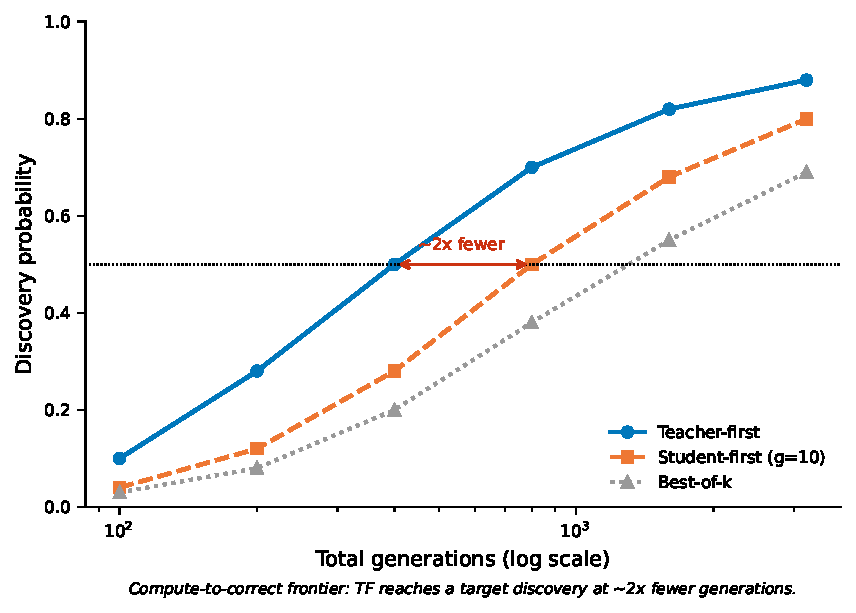
\includegraphics[width=\linewidth]{../figures/bc_fig3_ctc.pdf}
\column{0.42\textwidth}
\begin{itemize}
  \item Match the budget: student-first at \textbf{10 generations/step}.
  \item Teacher-first still wins, and reaches a target discovery with \alert{$\sim$2$\times$ fewer total generations}.
  \item The advantage is the \emph{kind} of distilled trajectory, not sample volume.
\end{itemize}
\end{columns}
\end{frame}

% 11
\begin{frame}{RQ2: epistemic suppression on code}
\begin{columns}
\column{0.58\textwidth}
\centering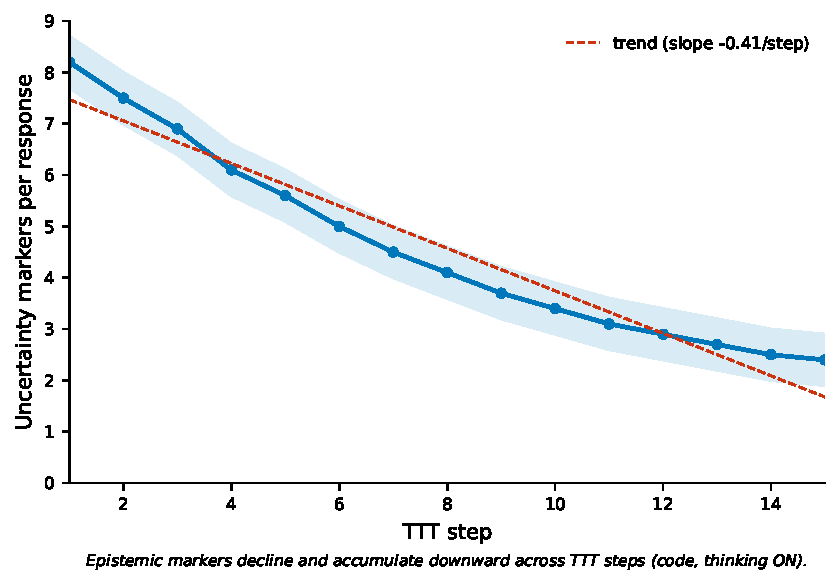
\includegraphics[width=\linewidth]{../figures/bc_fig4_epistemic.pdf}
\column{0.42\textwidth}
\begin{itemize}
  \item Uncertainty markers (``wait'', ``let me reconsider'') \textbf{decline} across steps, accumulating.
  \item Connects to Kim et al.: high $I(y;c\mid x)\Rightarrow$ suppression.
  \item \emph{On code} this coincides with \alert{improved} correctness --- consolidation, not answer-copying.
\end{itemize}
\end{columns}
\end{frame}

% 12
\begin{frame}{The central insight: value vs.\ procedure}
\begin{columns}
\column{0.58\textwidth}
\centering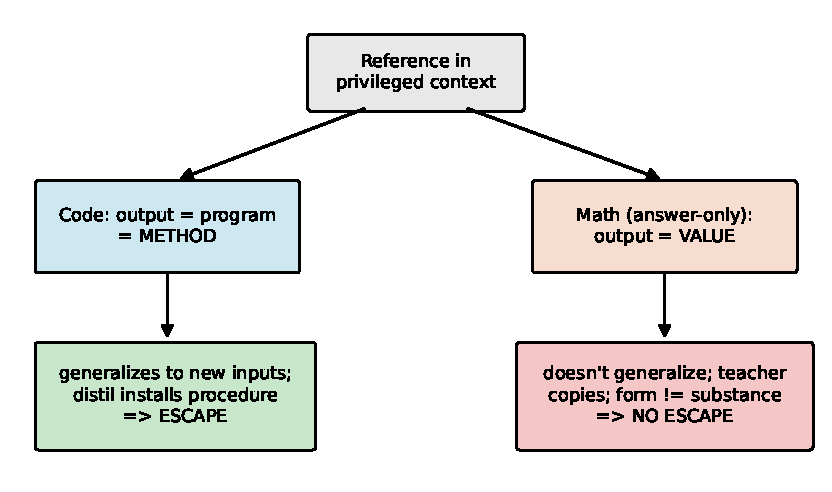
\includegraphics[width=\linewidth]{../figures/bc_fig5_boundary.pdf}
\column{0.42\textwidth}
\begin{itemize}
  \item Code output \emph{is} a method (a program that generalizes) $\Rightarrow$ distillation installs a procedure $\Rightarrow$ \textbf{escape}.
  \item Answer-only math output is a value $\Rightarrow$ the teacher can only copy $\Rightarrow$ \textbf{no escape}.
  \item Escape needs an \alert{in-reach method}, not merely a correct value.
\end{itemize}
\end{columns}
\end{frame}

% 13
\begin{frame}{Contributions}
\begin{enumerate}
  \item A \textbf{teacher-first} organization of execution-guided self-distillation (clean filter, never distils a copy).
  \item Teacher-first \textbf{significantly accelerates discovery} and \textbf{escapes the flat-reward trap} --- compute-fair (RQ3).
  \item A \textbf{reprompt-template effect}, strongest on hard problems (RQ1).
  \item A measured \textbf{epistemic-suppression} result on code (RQ2).
  \item A \textbf{value-versus-procedure boundary} characterizing \emph{when} the method helps.
\end{enumerate}
\end{frame}

% 14
\begin{frame}{Limitations \& publication roadmap}
\textbf{Honest bounds:} one 4B model family at a personal compute scale; a stronger model is expected to \emph{narrow} the margin; reward shape and reference content co-vary across domains.
\vfill
\textbf{Roadmap (a few months post-graduation):}
\begin{enumerate}
  \item medium-scale matched comparison $+$ compute-to-correct frontier;
  \item thinking-on code for the epistemic measurement;
  \item method-bearing math references (MATH-500) $+$ same reasoner;
  \item scale to 8B; second code benchmark.
\end{enumerate}
\end{frame}

% 15
\begin{frame}{Conclusion}
\begin{itemize}
  \item \textbf{Teacher-first execution-guided self-distillation} accelerates test-time discovery in complex code generation.
  \item It escapes the flat-reward trap, the advantage is \textbf{compute-fair}, and it carries a measured epistemic effect.
  \item The \textbf{value-versus-procedure boundary} explains \emph{when} it works: an in-reach method, not just an answer.
\end{itemize}
\vfill
\centering\Large Thank you. \normalsize\\[1em]
\small Questions?
\end{frame}

\end{document}
